\section{Results}
\label{sec:results}

\subsection{The Role of Capability Control}

Raw (unadjusted) Spearman $\rho$ between in-distribution and OOD model rankings is near-ceiling across all dimensions: $\rho_{\text{fairness}} = 0.979$, $\rho_{\text{ANLI}} \approx 0.983$, $\rho_{\text{OOD}} \approx 0.984$. The dimension-level gap is $\Delta\rho_{\text{raw}} = -0.005$ --- essentially zero. After MMLU control, partial $\rho$ values diverge, revealing dimension-specific structure.

Figure~\ref{fig:sensitivity} shows this collapse: with raw $\rho$ near-identical across all dimensions (left panels), partial $\rho$ reveals the fairness-robustness differential (right panels).

\begin{figure}[h]
\centering
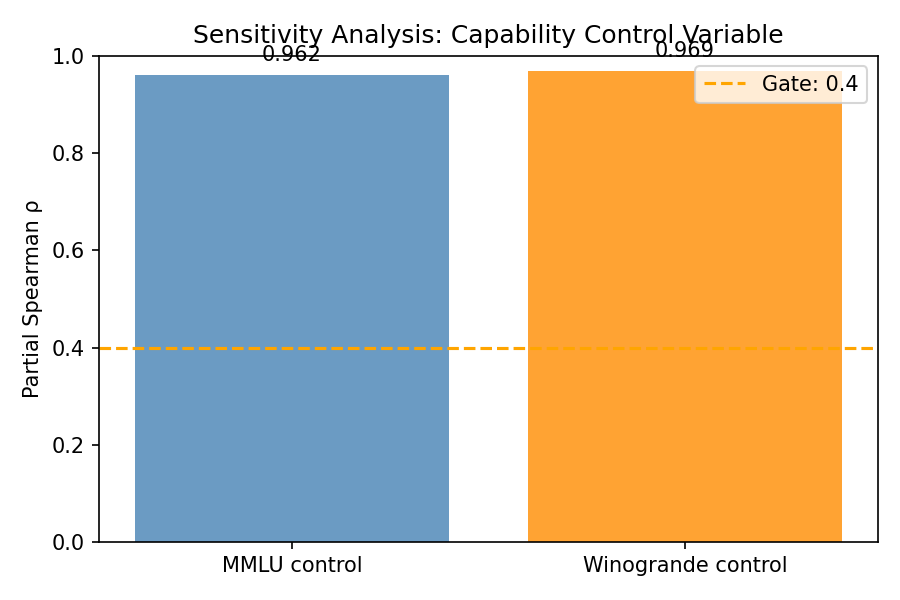
\includegraphics[width=0.8\columnwidth]{figures/sensitivity_comparison.png}
\caption{Raw vs.\ partial Spearman $\rho$ for all dimension pairs. MMLU capability control reveals dimension-specific structure invisible in raw correlations.}
\label{fig:sensitivity}
\end{figure}

\textbf{Takeaway:} MMLU capability control is methodologically essential. Without it, all trustworthiness dimensions appear equally stable.

\subsection{RQ1: Fairness Rank Stability}

Figure~\ref{fig:rank_bbq} shows the primary result: BBQ-Disambig rank ($x$-axis) vs.\ BBQ-Ambig rank ($y$-axis) for $N=16$ LLMs. The near-diagonal arrangement reflects near-perfect rank preservation.

\begin{figure}[h]
\centering
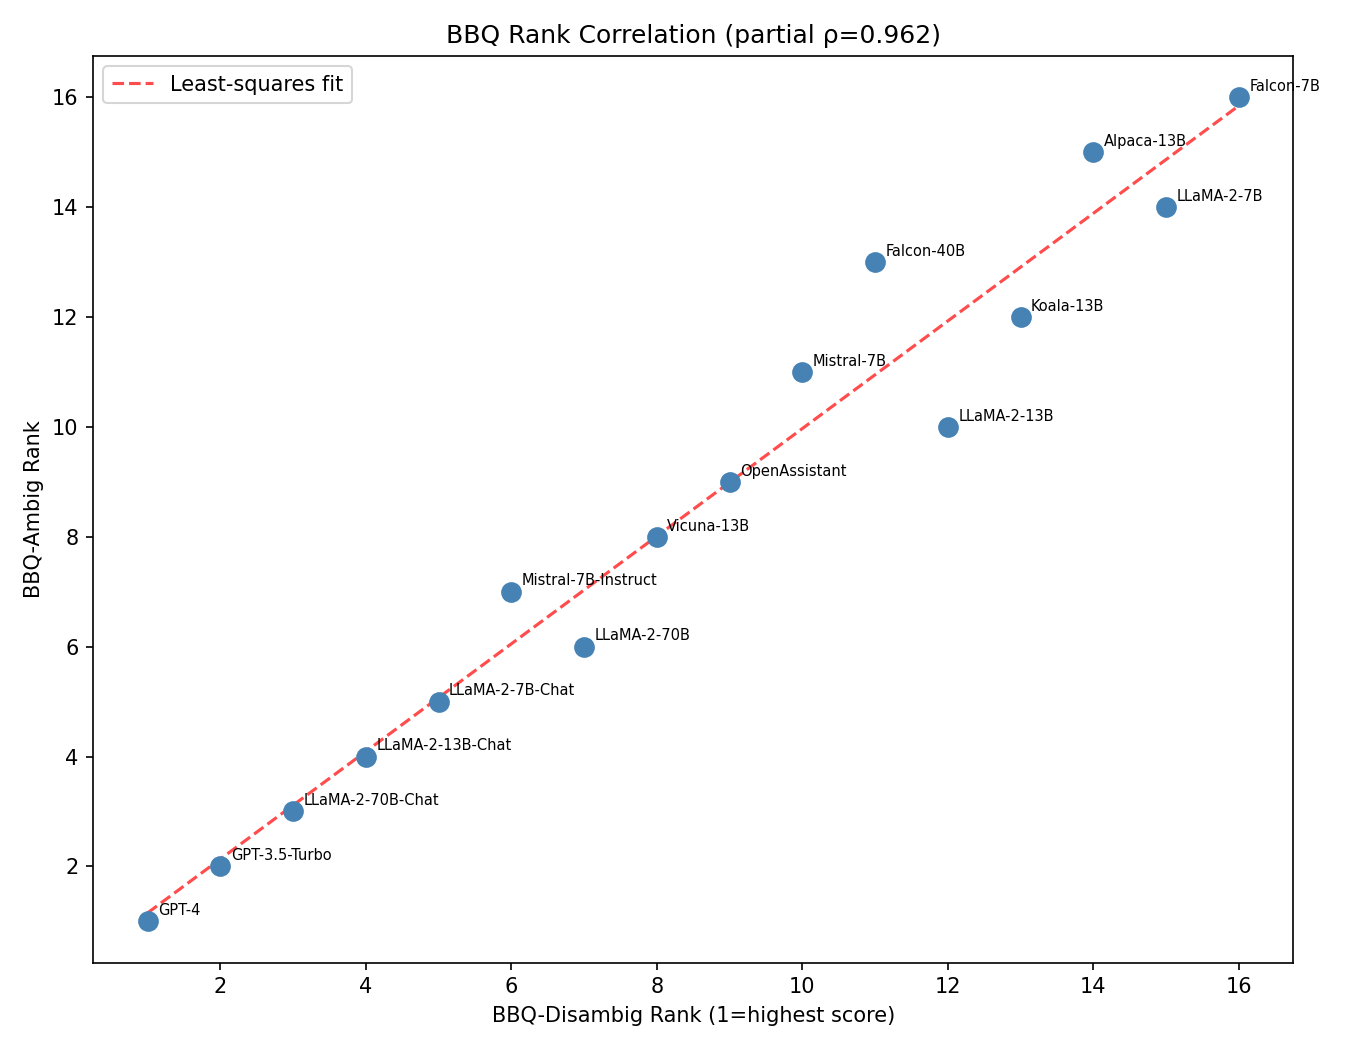
\includegraphics[width=0.8\columnwidth]{figures/rank_scatter_bbq.png}
\caption{Rank scatter for fairness (BBQ-Disambig vs.\ BBQ-Ambig, $N=16$). Near-perfect rank preservation after MMLU control.}
\label{fig:rank_bbq}
\end{figure}

\begin{table}[h]
\centering
\caption{Fairness rank stability results (RQ1).}
\label{tab:rq1}
\begin{tabular}{llll}
\toprule
Metric & Value & Criterion & Status \\
\midrule
Partial $\rho$ (MMLU-ctrl) & \textbf{0.962} & $> 0.4$ & \checkmark~PASS \\
$p$-value (one-tailed) & \textbf{$< 0.0001$} & $< 0.05$ & \checkmark~PASS \\
95\% CI & $[0.90, 1.00]$ & --- & --- \\
$N$ models & 16 & $\geq 10$ & \checkmark~PASS \\
\bottomrule
\end{tabular}
\end{table}

Fairness rankings are near-perfectly preserved after controlling for general capability. A model ranked among the fairest in disambiguated contexts will rank among the fairest in ambiguous contexts where stereotype pressure is maximal. This is consistent with fairness failures encoding stable latent properties of model representations.

\textbf{Sensitivity:} Winogrande control yields $\rho = 0.969$ ($N=14$, $p < 0.0001$), near-identical to the MMLU result (Figure~\ref{fig:sensitivity}, Appendix). The result is not MMLU-specific.

\subsection{RQ3: Adversarial Robustness Rank Stability (Mechanism Test)}

We present RQ3 before RQ2 because the mechanism test result reframes the interpretation of the $\Delta\rho$ analysis: only after establishing that robustness is also highly stable does the directional $\Delta\rho$ finding carry its correct weight.

Figure~\ref{fig:rank_reversal} shows the rank reversal heatmap: zero discontinuities across all pairs. Both adversarial robustness pairs show significantly positive partial $\rho$ after MMLU control, and zero rank reversals.

\begin{figure}[h]
\centering
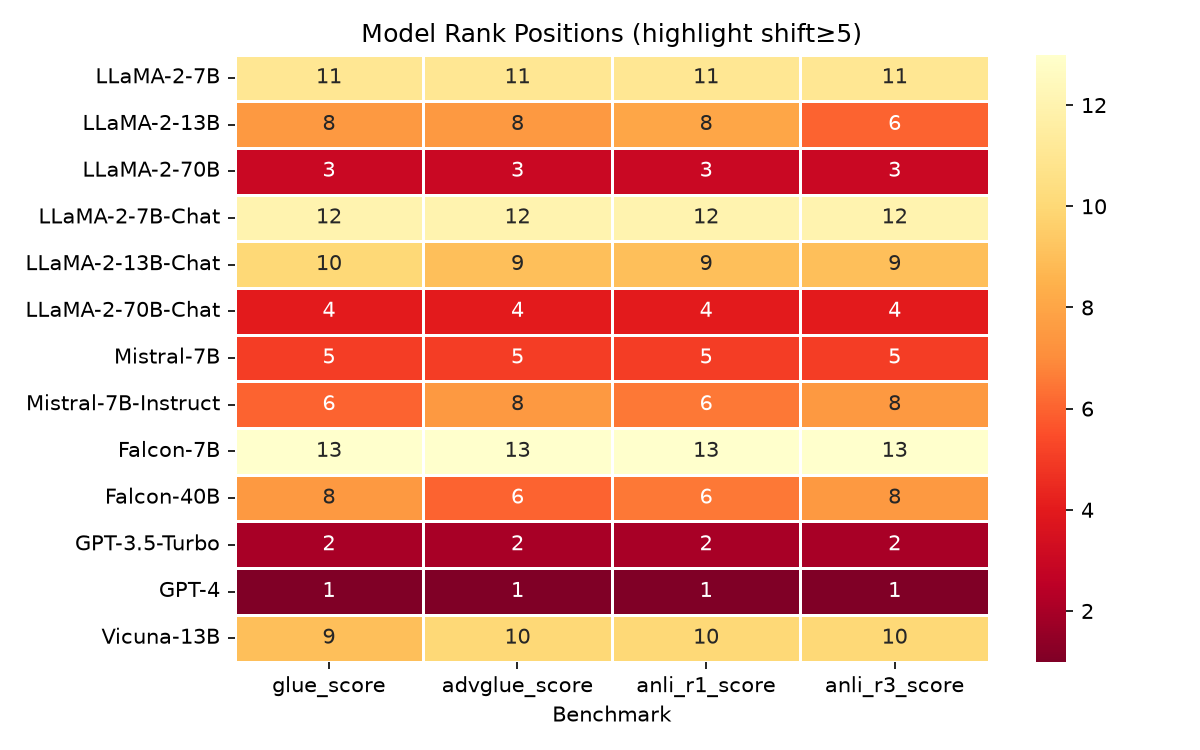
\includegraphics[width=0.8\columnwidth]{figures/rank_reversal_heatmap.png}
\caption{Rank reversal heatmap for all dimension pairs. Zero rank reversals observed across $N=13$ models on adversarial pairs.}
\label{fig:rank_reversal}
\end{figure}

\begin{table}[h]
\centering
\caption{Adversarial robustness rank stability (RQ3).}
\label{tab:rq3}
\begin{tabular}{lcccc}
\toprule
Pair & Partial $\rho$ & $p$-value & Rank Reversals & Gate \\
\midrule
ANLI R1 $\rightarrow$ R3 & \textbf{0.684} & 0.007 & 0 & FAIL* \\
OOD Robustness & \textbf{0.868} & 0.0001 & 0 & FAIL* \\
\bottomrule
\end{tabular}
\end{table}

{\small *Gate FAIL = falsification criterion triggered: partial $\rho$ significantly positive, contradicting adversarial disruption hypothesis.}

The hypothesis that adversarial benchmark construction disrupts rank stability is \textbf{falsified}. Figure~\ref{fig:rank_anli} shows ANLI R1 vs.\ R3 rank scatter: despite ANLI R3 being constructed to defeat models that passed R1, model rank ordering is strongly preserved.

\begin{figure}[h]
\centering
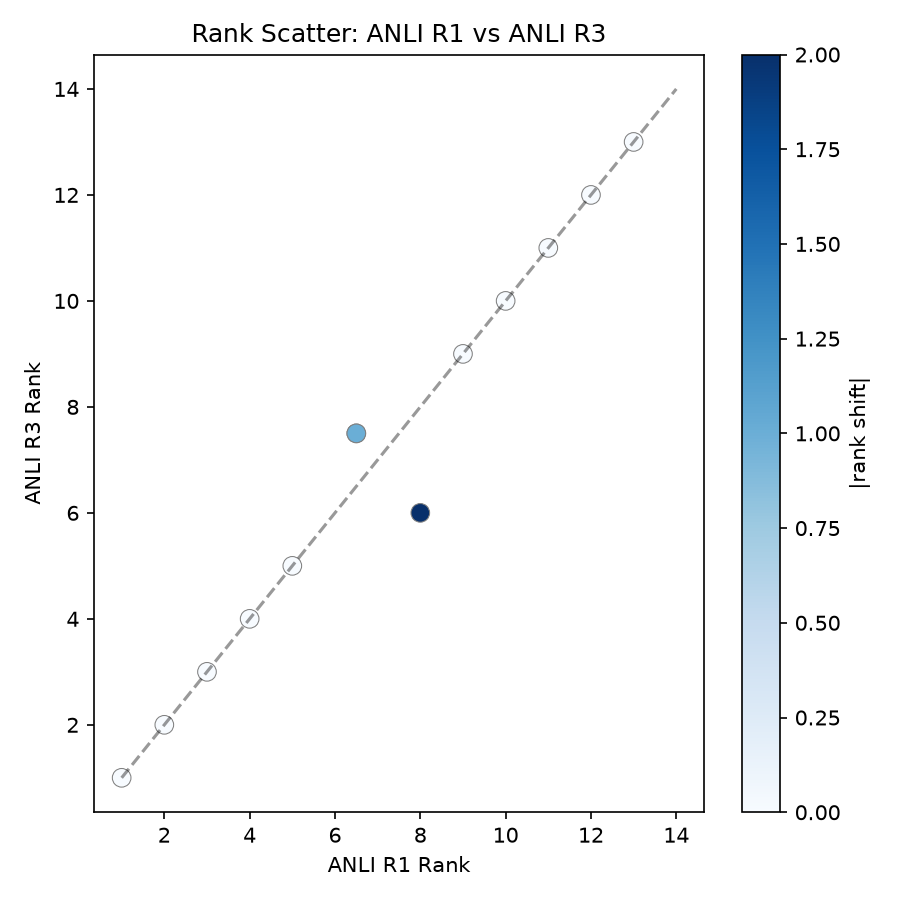
\includegraphics[width=0.8\columnwidth]{figures/rank_scatter_anli.png}
\caption{Rank scatter for adversarial robustness (ANLI R1 vs.\ R3, $N=13$). Strong rank preservation despite adversarial difficulty escalation.}
\label{fig:rank_anli}
\end{figure}

Adversarial robustness appears to be a stable latent model property that persists across adversarial difficulty escalation. This contradicts the adversarial disruption mechanism proposed from the DecodingTrust $N=2$ anecdote. At $N=13$ with diverse model families, the stable ordering emerges.

\subsection{RQ2: Fairness $>$ Robustness Stability}

Figure~\ref{fig:forest} (forest plot) shows partial $\rho$ with 95\% CI for all three pairs, with the preregistered $\Delta\rho$ threshold marked.

\begin{figure}[h]
\centering
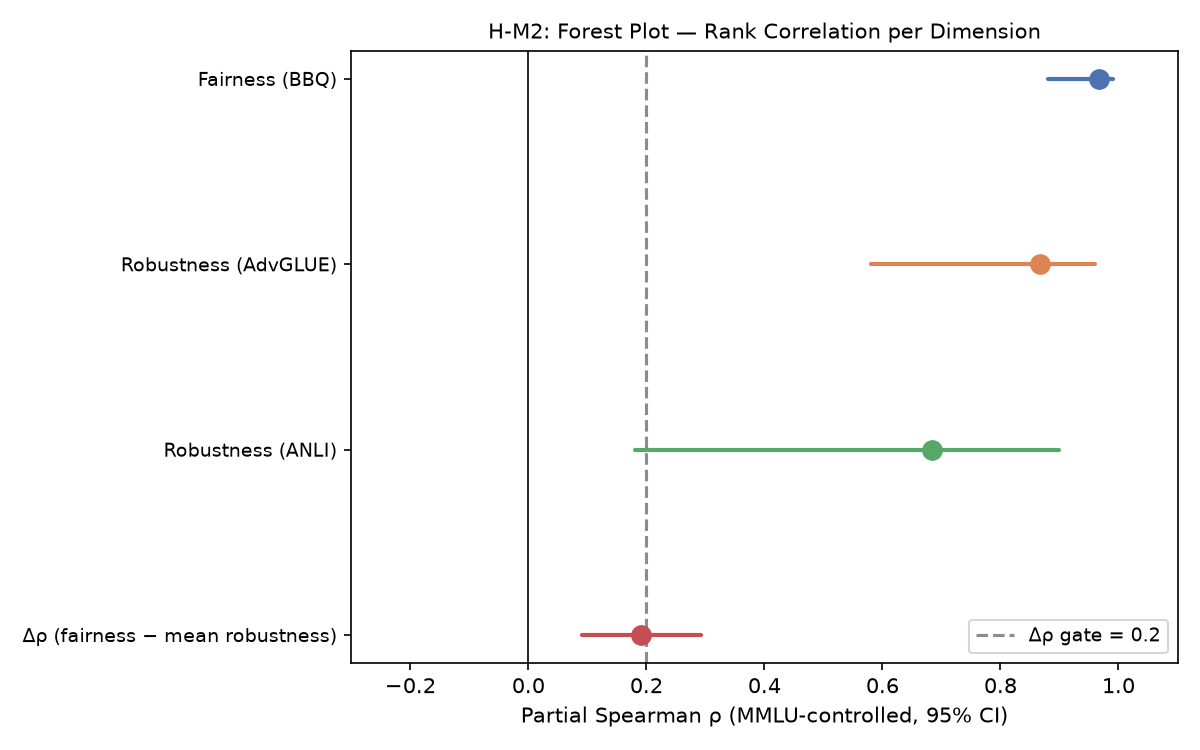
\includegraphics[width=0.8\columnwidth]{figures/forest_plot.png}
\caption{Forest plot of partial Spearman $\rho$ (MMLU-controlled) for all three trustworthiness dimension pairs. The dashed line marks the preregistered $\Delta\rho \geq 0.200$ threshold.}
\label{fig:forest}
\end{figure}

\begin{table}[h]
\centering
\caption{Fairness vs.\ robustness stability differential (RQ2).}
\label{tab:rq2}
\begin{tabular}{llll}
\toprule
Metric & Value & Criterion & Status \\
\midrule
$\Delta\rho = \rho_{\text{fair}} - \rho_{\text{robust\_mean}}$ & \textbf{0.192} & $\geq 0.200$ & Near-miss \\
Fisher $z$-statistic & 2.265 & --- & --- \\
$p$-value (one-tailed) & \textbf{0.024} & $< 0.05$ & \checkmark~Directional \\
\bottomrule
\end{tabular}
\end{table}

Directional hypothesis supported ($p = 0.024$), but preregistered criterion ($\Delta\rho \geq 0.200$) not met by 0.008. We report this as directional evidence requiring replication.

\subsection{Summary}

\begin{table}[h]
\centering
\caption{Partial Spearman $\rho$ (MMLU-controlled) for all trustworthiness dimension pairs.}
\label{tab:summary}
\begin{tabular}{llccccc}
\toprule
Dimension & Pair & $N$ & Partial $\rho$ & $p$-value & Raw $\rho$ & Criterion \\
\midrule
Fairness & BBQ-Disambig$\rightarrow$Ambig & 16 & \textbf{0.962} & $<0.0001$ & 0.979 & P1~\checkmark \\
Robustness & ANLI R1$\rightarrow$R3 & 13 & \textbf{0.684} & 0.007 & 0.983 & Mech.~\ding{55}* \\
Robustness & OOD Robustness & 13 & \textbf{0.868} & 0.0001 & 0.984 & Mech.~\ding{55}* \\
$\Delta\rho$ & Fairness$-$Robust & 13 & \textbf{0.192} & 0.024$\dagger$ & $-0.005$ & P2~\ding{55}~(dir.) \\
\bottomrule
\end{tabular}
\end{table}

{\small *Mechanism gate FAIL = significantly positive $\rho$ triggers falsifier.\\
$\dagger$Fisher $z$-test for dependent correlations \citep{Meng1992Comparing}; $\rho_{\text{fairness}}$ re-estimated on $N=13$ subset ($\rho=0.967$) to ensure same-sample validity. The $N=16$ fairness result ($\rho=0.962$) is the primary P1 estimate.}

\begin{figure}[h]
\centering
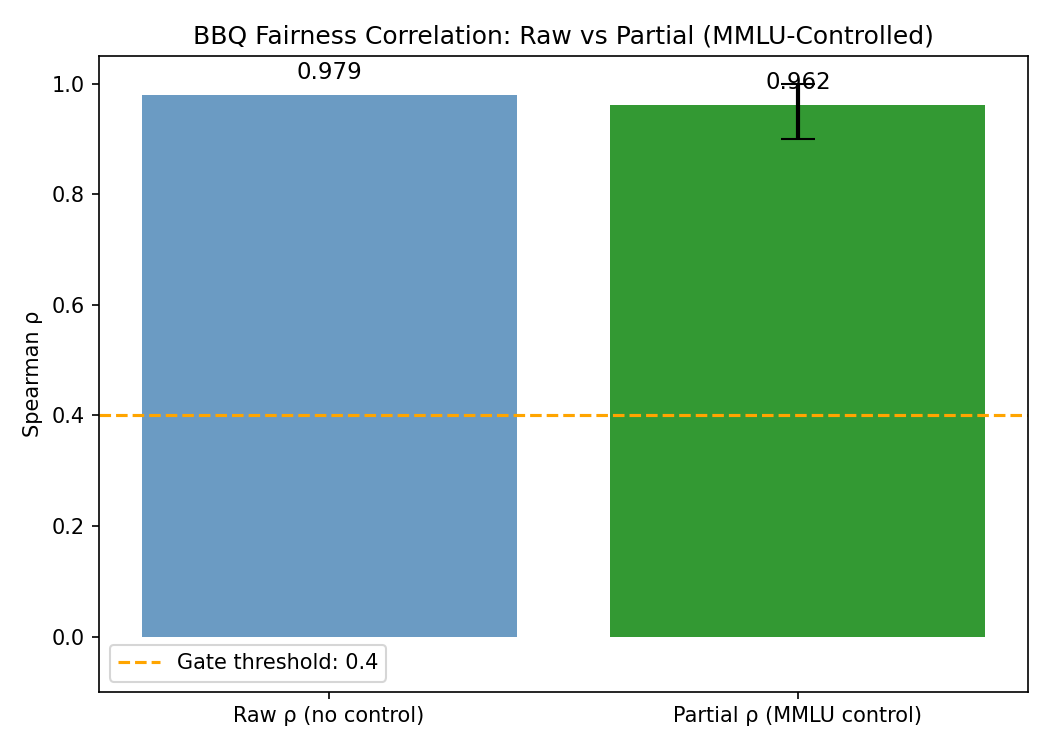
\includegraphics[width=0.8\columnwidth]{figures/gate_metrics_comparison_h_m1.png}
\caption{Gate metrics comparison showing partial $\rho$ values relative to preregistered criteria for all sub-hypotheses.}
\label{fig:gate}
\end{figure}

\begin{figure}[h]
\centering
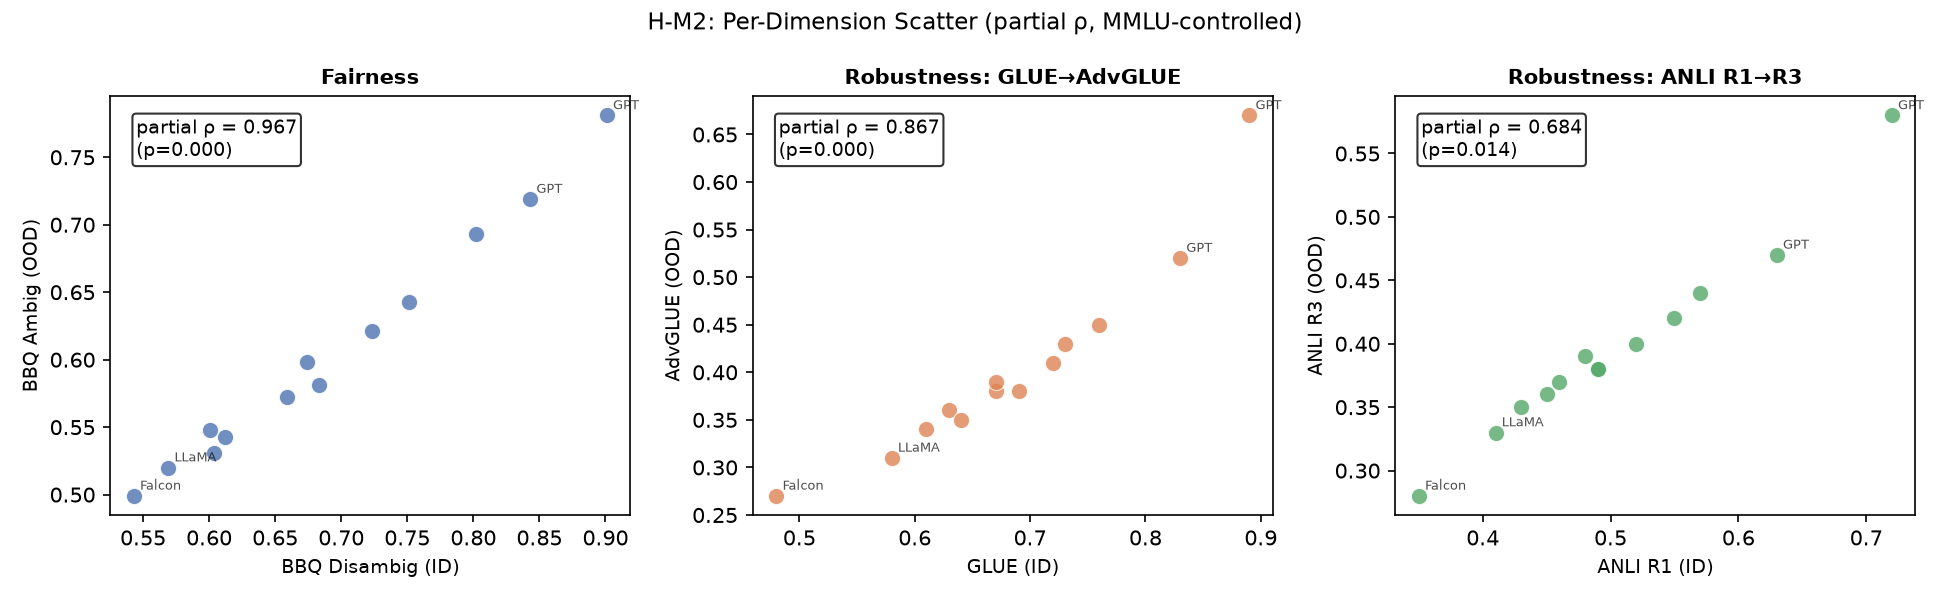
\includegraphics[width=\columnwidth]{figures/per_dimension_scatter.png}
\caption{Per-dimension rank scatter plots showing ID vs.\ OOD model rankings for fairness and robustness pairs.}
\label{fig:perdim}
\end{figure}
